%%%%%%%%%%%%%%%%%%%%%%%%%%%%%%%%%%%%%%%%%
% Lachaise Assignment
% LaTeX Template
% Version 1.0 (26/6/2018)
%
% This template originates from:
% http://www.LaTeXTemplates.com
%
% Authors:
% Marion Lachaise & Fran\UTF{00C3}§ois F\UTF{00C3}\UTF{00A9}votte
% Vel (vel@LaTeXTemplates.com)
%
% License:
% CC BY-NC-SA 3.0 (http://creativecommons.org/licenses/by-nc-sa/3.0/)
% 
%%%%%%%%%%%%%%%%%%%%%%%%%%%%%%%%%%%%%%%%%

%----------------------------------------------------------------------------------------
%	PACKAGES AND OTHER DOCUMENT CONFIGURATIONS
%----------------------------------------------------------------------------------------

\documentclass{article}
%German language
\usepackage[ngerman]{babel}
\usepackage[utf8]{inputenc}
\usepackage[T1]{fontenc} 
\usepackage{cancel}
\usepackage{xifthen}
\usepackage{venndiagram}
\usepackage{pgfplots}
\usepackage{wrapfig}
\usepackage{comment}
\usepackage{amsmath}
\usepackage[nolist]{acronym}
\usepackage{xcolor}
\usepackage{algorithmic}
\usepackage{multicol}
\usepackage{csquotes}
\usepackage{tikz}
\usepackage{hyperref}
\usetikzlibrary{calc,shapes.multipart,chains,arrows}
\usepackage{titlesec}


\usepackage{listings}
\usepackage{xcolor}

\definecolor{codegreen}{rgb}{0,0.6,0}
\definecolor{codegray}{rgb}{0.5,0.5,0.5}
\definecolor{codepurple}{rgb}{0.58,0,0.82}
\definecolor{backcolour}{rgb}{0.95,0.95,0.92}

\lstdefinestyle{mystyle}{
	backgroundcolor=\color{backcolour},   
	commentstyle=\color{codegreen},
	keywordstyle=\color{magenta},
	numberstyle=\tiny\color{codegray},
	stringstyle=\color{codepurple},
	basicstyle=\ttfamily\footnotesize,
	breakatwhitespace=false,         
	breaklines=true,                 
	captionpos=b,                    
	keepspaces=true,                 
	numbers=left,                    
	numbersep=5pt,                  
	showspaces=false,                
	showstringspaces=false,
	showtabs=false,                  
	tabsize=2
}

\lstset{style=mystyle}


%%%%%%%%%%%%%%%%%%%%%%%%%%%%%%%%%%%%%%%%%
% Lachaise Assignment
% Structure Specification File
% Version 1.0 (26/6/2018)
%
% This template originates from:
% http://www.LaTeXTemplates.com
%
% Authors:
% Marion Lachaise & François Févotte
% Vel (vel@LaTeXTemplates.com)
%
% License:
% CC BY-NC-SA 3.0 (http://creativecommons.org/licenses/by-nc-sa/3.0/)
% 
%%%%%%%%%%%%%%%%%%%%%%%%%%%%%%%%%%%%%%%%%

%----------------------------------------------------------------------------------------
%	PACKAGES AND OTHER DOCUMENT CONFIGURATIONS
%----------------------------------------------------------------------------------------

\usepackage{amsmath,amsfonts,stmaryrd,amssymb} % Math packages

\usepackage{enumerate} % Custom item numbers for enumerations

\usepackage[ruled]{algorithm2e} % Algorithms

\usepackage[framemethod=tikz]{mdframed} % Allows defining custom boxed/framed environments

\usepackage{listings} % File listings, with syntax highlighting
\lstset{
	basicstyle=\ttfamily, % Typeset listings in monospace font
}

%----------------------------------------------------------------------------------------
%	DOCUMENT MARGINS
%----------------------------------------------------------------------------------------

\usepackage{geometry} % Required for adjusting page dimensions and margins

\geometry{
	paper=a4paper, % Paper size, change to letterpaper for US letter size
	top=2.5cm, % Top margin
	bottom=3cm, % Bottom margin
	left=2.5cm, % Left margin
	right=2.5cm, % Right margin
	headheight=14pt, % Header height
	footskip=1.5cm, % Space from the bottom margin to the baseline of the footer
	headsep=1.2cm, % Space from the top margin to the baseline of the header
	%showframe, % Uncomment to show how the type block is set on the page
}

%----------------------------------------------------------------------------------------
%	FONTS
%----------------------------------------------------------------------------------------

\usepackage[utf8]{inputenc} % Required for inputting international characters
\usepackage[T1]{fontenc} % Output font encoding for international characters

\usepackage{XCharter} % Use the XCharter fonts

%----------------------------------------------------------------------------------------
%	COMMAND LINE ENVIRONMENT
%----------------------------------------------------------------------------------------

% Usage:
% \begin{commandline}
%	\begin{verbatim}
%		$ ls
%		
%		Applications	Desktop	...
%	\end{verbatim}
% \end{commandline}

\mdfdefinestyle{commandline}{
	leftmargin=10pt,
	rightmargin=10pt,
	innerleftmargin=15pt,
	middlelinecolor=black!50!white,
	middlelinewidth=2pt,
	frametitlerule=false,
	backgroundcolor=black!5!white,
	frametitle={Command Line},
	frametitlefont={\normalfont\sffamily\color{white}\hspace{-1em}},
	frametitlebackgroundcolor=black!50!white,
	nobreak,
}

% Define a custom environment for command-line snapshots
\newenvironment{commandline}{
	\medskip
	\begin{mdframed}[style=commandline]
}{
	\end{mdframed}
	\medskip
}

%----------------------------------------------------------------------------------------
%	FILE CONTENTS ENVIRONMENT
%----------------------------------------------------------------------------------------

% Usage:
% \begin{file}[optional filename, defaults to "File"]
%	File contents, for example, with a listings environment
% \end{file}

\mdfdefinestyle{file}{
	innertopmargin=1.6\baselineskip,
	innerbottommargin=0.8\baselineskip,
	topline=false, bottomline=false,
	leftline=false, rightline=false,
	leftmargin=2cm,
	rightmargin=2cm,
	singleextra={%
		\draw[fill=black!10!white](P)++(0,-1.2em)rectangle(P-|O);
		\node[anchor=north west]
		at(P-|O){\ttfamily\mdfilename};
		%
		\def\l{3em}
		\draw(O-|P)++(-\l,0)--++(\l,\l)--(P)--(P-|O)--(O)--cycle;
		\draw(O-|P)++(-\l,0)--++(0,\l)--++(\l,0);
	},
	nobreak,
}

% Define a custom environment for file contents
\newenvironment{file}[1][File]{ % Set the default filename to "File"
	\medskip
	\newcommand{\mdfilename}{#1}
	\begin{mdframed}[style=file]
}{
	\end{mdframed}
	\medskip
}

%----------------------------------------------------------------------------------------
%	NUMBERED QUESTIONS ENVIRONMENT
%----------------------------------------------------------------------------------------

% Usage:
% \begin{question}[optional title]
%	Question contents
% \end{question}

\mdfdefinestyle{question}{
	innertopmargin=1.2\baselineskip,
	innerbottommargin=0.8\baselineskip,
	roundcorner=5pt,
	nobreak,
	singleextra={%
		\draw(P-|O)node[xshift=1em,anchor=west,fill=white,draw,rounded corners=5pt]{%
		\questionTitle};
	},
}

\newcounter{Question} % Stores the current question number that gets iterated with each new question

% Define a custom environment for numbered questions
\newenvironment{question}[1][\unskip]{
	\bigskip
	\stepcounter{Question}
	\newcommand{\questionTitle}{~#1}
	\begin{mdframed}[style=question]
}{
	\end{mdframed}
	\medskip
}

%----------------------------------------------------------------------------------------
%	WARNING TEXT ENVIRONMENT
%----------------------------------------------------------------------------------------

% Usage:
% \begin{warn}[optional title, defaults to "Warning:"]
%	Contents
% \end{warn}

\mdfdefinestyle{warning}{
	topline=false, bottomline=false,
	leftline=false, rightline=false,
	nobreak,
	singleextra={%
		\draw(P-|O)++(-0.5em,0)node(tmp1){};
		\draw(P-|O)++(0.5em,0)node(tmp2){};
		\fill[black,rotate around={45:(P-|O)}](tmp1)rectangle(tmp2);
		\node at(P-|O){\color{white}\scriptsize\bf !};
		\draw[very thick](P-|O)++(0,-1em)--(O);%--(O-|P);
	}
}

% Define a custom environment for warning text
\newenvironment{warn}[1][Warning:]{ % Set the default warning to "Warning:"
	\medskip
	\begin{mdframed}[style=warning]
		\noindent{\textbf{#1}}
}{
	\end{mdframed}
}

%----------------------------------------------------------------------------------------
%	INFORMATION ENVIRONMENT
%----------------------------------------------------------------------------------------

% Usage:
% \begin{info}[optional title, defaults to "Info:"]
% 	contents
% 	\end{info}

\mdfdefinestyle{info}{%
	topline=false, bottomline=false,
	leftline=false, rightline=false,
	nobreak,
	singleextra={%
		\fill[black](P-|O)circle[radius=0.4em];
		\node at(P-|O){\color{white}\scriptsize\bf i};
		\draw[very thick](P-|O)++(0,-0.8em)--(O);%--(O-|P);
	}
}

% Define a custom environment for information
\newenvironment{info}[1][Info:]{ % Set the default title to "Info:"
	\medskip
	\begin{mdframed}[style=info]
		\noindent{\textbf{#1}}
}{
	\end{mdframed}
}
 % Include the file specifying the document structure and custom commands
%----------------------------------------------------------------------------------------
%	ASSIGNMENT INFORMATION
%----------------------------------------------------------------------------------------

\title{GDPR Compliant Cloud Data Storage and Processing Engine as a Service\\[0.4em]\smaller{}\smaller{}Cryptographic Protocols} 
\author{
	Mats Kockmeyer\\ \texttt{Mats.Kockmeyer2@stud.hs-flensburg.de}\\\\
	Felix Janke\\ \texttt{Felix.Janke2@stud.hs-flensburg.de}
} 

\date{Hochschule Flensburg --- \today} % University, school and/or department name(s) and a date

%----------------------------------------------------------------------------------------
\allowdisplaybreaks
\definecolor{light}{RGB}{138, 216, 203}
\begin{document}
\begin{acronym}
\acro{CSP}{Cloud Service Provider}
\acro{DRAM}{Dynamic Random Access Memory}
\acro{PRM}{Processor Reserved Memory}
\acro{EPC}{Enclave Page Cache}
\acro{SQL}{Structured Query Language}
\end{acronym}

\maketitle % Print the title

\newcommand{\acr}[1]{\acs{#1} (\aclu{#1})}

 \newcommand{\wip}[1]{
  \ifthenelse{\isempty{#1}}%
    {\colorbox{yellow!50}{$\boxast $}}% if #1 is empty
    {\colorbox{yellow!50}{$\boxast $}\textit{\smaller{} #1} }% if #1 is not empty
   }


%Input sections
\section{Projekt}
Das Ziel des Projektes ist es, eine Möglichkeit zur GDPR Konformen Verarbeitung von personenbezogenen Daten in der Cloud zu finden. Nach Möglichkeiten sollen die personenbezogenen Daten anonymisiert außerhalb der Europäischen Union gespeichert und verarbeitet werden.  Sind die Daten anonymisiert gespeichert, muss mit der entsprechenden Firma kein Datenverarbeitungsauftrag ausgehandelt werden, da dies nicht unter die Anwendungsbereich (Artike 2, weiter Artikel 4) der GDPR fällt.


\section{Firmen Definition}
Der Service soll Exemplarisch anhand einer Firma erklärt und durchgeführt werden. Zuerst muss die Firma dafür definiert werden.\\\\

\begin{table}[h!]
\centering
\begin{tabular}{l|c}
Branche           & KFZ Gewerbe                   \\ \hline
Land              & Deutschland                   \\ \hline
Standorte         & 1                             \\ \hline
Betriebsgröße     & 120 Mitarbeiter               \\ \hline
Kundenstamm       & 50.000                        \\ \hline
Datenbankgröße    & 100 GiB                       \\ \hline
Infrastruktur     & Lokale                        \\ \hline
Internetanbindung & 100 MBits Down \& 40 MBits Up
\end{tabular}
\end{table} 

Zum aktuellen Zeitpunkt werden die personenbezogenen Daten in der Firma, in einer getrennten Räumlichkeit, auf einem lokalen Server gespeichert. Um Kosten und eventuelle Ausfallzeiten zu minimieren, sollen die Daten zu einem Cloud Anbieter migriert werden. Aufgrund der hohen kosten deutscher Cloud Anbieter, würde Firma eine Speicherung in einer Ausländischen Cloud bevorzugen, zum Beispiel in Russland.
\section{Anforderungen}
In diesem Kapitel werden die Anforderung an den Cloud Service zusammengefasst.

\begin{itemize}
\item Einhalterung der GDPR.
\item Speicherung der Daten außerhalb der EU.
\item Verschlüsselung muss als Anonymisierung gelten.
\item Die Daten müssen für externe Firmen als anonymisiert gelten, damit diese nicht unter die GDPR fallen. 
\item Bereits bei der Kommunikation von der Firma in die Cloud, müssen die Daten als anonymisiert gelten2. 
\end{itemize}
\section{Architektur}
Für die Realisierung der GDPR konformen Datenverarbeitung ohne die Erteilung eines Verarbeitungsauftrages an das jeweilige \ac{CSP} soll Intel SGX eingesetzt werden. Intel SGX bietet die Möglichkeit gesicherte Programmbereiche auszuführen, sodass von extern kein Zugriff möglich ist. Diese Funktionsweise bildet die geschützte Datenverarbeitung innerhalb eines Rechenzentrums ab, ohne eine Zugriffsmöglichkeit direkt von anderen Instanzen auf der physikalischen Maschine sowie den indirekten Zugriff über die Infrastruktur durch das \ac{CSP}. 

In \autoref{img:sgx-idea} ist der Aufbau skizziert. Der grüne Bereich repräsentiert hierbei den vertrauenswürdigen Bereich und die direkte Zuständigkeit eines beliebigen Unternehmens. Auf der rechten Seite ist dieses Unternehm abgebildet, welches über verschiedene Clients verfügt und über eine gesicherte Verbindung auf den Datencontainer bei einen Hosting Container zugreifen möchte. 

\begin{figure}[h!]
	\centering
	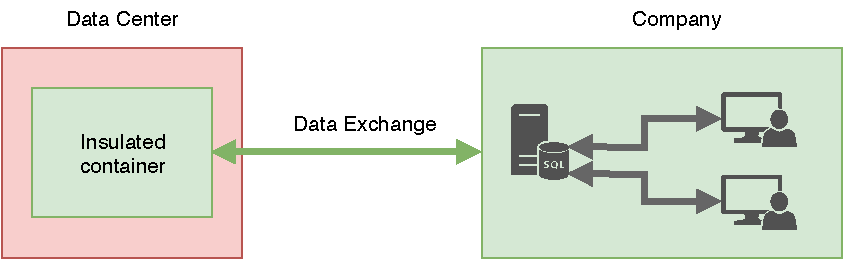
\includegraphics{img/sgx_idea/sgx-idea.pdf}
	\caption{Skizzierung des Ziels einer gesicherten Umgebung bei einem \ac{CSP}}
	\label{img:sgx-idea}
\end{figure}

\subsection{Intel SGX}
 In diesem Abschnitt werden lediglich die wichtigsten Komponenten beschrieben, welche für das Verständnis der Architektur notwendig sind. Intel SGX ermöglicht die Bereitstellung von sicheren Programmumgebungen, die sogenannten \emph{Enclaves}. Eine Enclave besteht aus zwei essentiellen Bestandteilen. Das Rahmenwerk einer Enclave definiert der \emph{Unsecure Part},  welcher keinerlei Schutzfunktionen unterliegt, jedoch die Schnittstellen zu dem eigentlichen, gesicherten Container innerhalb einer Enclave beinhaltet.
 
 Die Enclaven werden innerhalb dem \ac{DRAM} abgelegt. In diesem existiert ein zusammenhängender Speicherbeich, welche den sogenannten \ac{PRM} beinhaltet. Auf diesen Bereich kann durch die Software nicht direkt zugegriffen werden. Der \ac{PRM} beinhaltet wiederum einen Speicherbereich, welcher \ac{EPC} bezeichnet wird. Der \ac{EPC} enthält alle Enclaves, die auf dem jeweiligen System agieren \cite{sgx-bibel}. Hierbei ist zu erwähnen, dass die parallele Ausführung mehrere Enclaves möglich ist.
 
 Die maximale Größe des \acs{EPC} beträgt 128 MiB. Hiervon können 93 MiB aktiv genutzt werden. Übersteigt eine Enclave die genannte Größe, so ist das kostspielige Swapping über den \ac{EPC} notwendig. \cite{sgx-performance} Programme, die innerhalb einer Enclave ausgeführt werden können, sind in den Programmiersprachen \emph{C} oder \emph{C++} zu schreiben. Zudem ist es grundsätzlich möglich beliebige Programmbibliotheken der jeweiligen Programmiersprache zu importieren.
 
 \subsection{Struktur einer Enclave}
 In diesem Abschnitt die die Struktur der Enclave betrachtet werden, welche genutzt wird, um Anfragen zu bearbeiten. Der erwähnte Use-Case ist das Handling von Datenbankoperationen auf einer verschlüsselten \ac{SQL} Datenbank. Das Interface für die gesicherte, externe Kommunikation wird zunächst abstrahiert. Es wird davon ausgegangen, dass die \ac{SQL} Instruktionen über ein sicheres Verfahren die Enclave erreichen. Diese stellt hierfür ein External Interface bereit. Diese Interface wird innerhalb des \emph{Unsicheren Bereichs} ausgeführt. Die Datenkommunikation dient hierbei lediglich als Relay und wird an das \emph{Communication Interface} des sicheren Bereichs weitergeleitet. \\
 
 
 Anschließend wird mit der $EncryptionEngine_{External}$ die Anfrage entschlüsselt und die extrahierten Instruktionen an den \emph{SQL Handler} weitergereicht. Parallel wird eine Anfrage an die $EncryptionEngine_{Storage}$ gestellt, welche die erforderlichen Daten anfragt. Auf Grund der möglichen Dimensionen einer Datenbank, muss diese außerhalb des sicheren Container gespeichert werden. Daraus resultiert, dass die Datenbank verschlüsselt werden muss, sodass keine Daten im Klartext die sichere Enclave verlassen. Die $EncryptionEngine_{Storage}$ fordert daher die Datenbank über den \emph{Perstistence Storage Handler} an und übernimmt die Entschlüsselung der Daten. Die Daten werden anschließend dem \emph{\ac{SQL} Handler} im Klartext zugeführt, sodass die angefragte Instruktion darauf angewendet werden kann. \\
 
 
 Nach der erfolgreichen Anwendung werden die neuen Datensätze über die $EncryptionEngine_{Storage}$ und den \emph{Perstistence Storage Handler} gesichert. Ergänzend dazu werden die Ergebnisse der Anfrage über die $EncryptionEngine_{External}$ und das \emph{Communication Interface} an den Kunden zurück gesendet.
 
 
 \begin{figure}[h!]
 	\centering
 	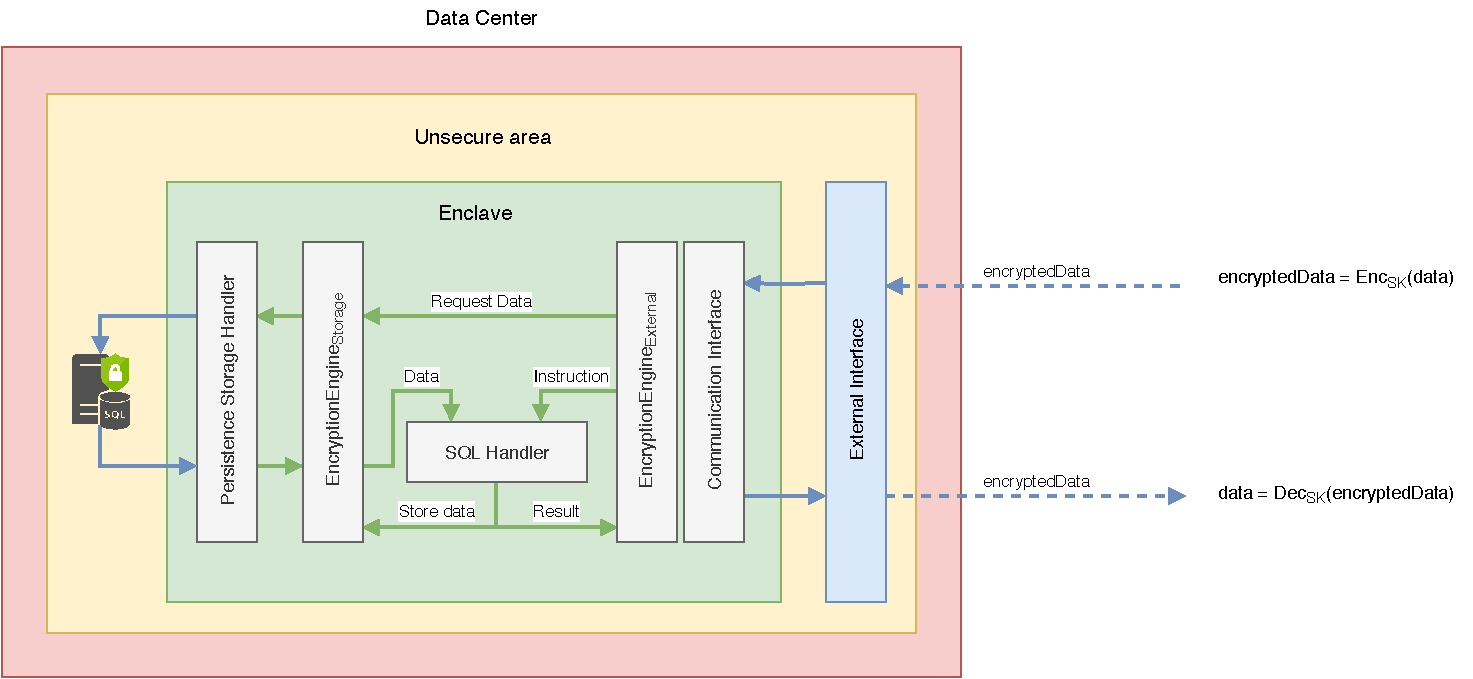
\includegraphics[width=0.8\textwidth]{img/enclave_details/enclave_details.pdf}
 	\caption{Skizzierung des Ziels einer gesicherten Umgebung bei einem \ac{CSP}}
 	\label{img:sgx-idea}
 \end{figure}
%------------------------------------------------
\begin{thebibliography}{9}
%\bibitem{blsPaper}
%Boneh, D., Drijvers, M., \& Neven, G. BLS Multi-Signatures With Public-Key Aggregation.	
\bibitem{sgx-bibel}
Costan, Victor, and Srinivas Devadas. 2016. Intel SGX Explained. http://eprint.iacr.org/2016/086 (November 8, 2019).

\bibitem{sgx-performance}
Weichbrodt, Nico, Pierre-Louis Aublin, and Rüdiger Kapitza. 2018. “Sgx-Perf: A Performance Analysis Tool for Intel SGX Enclaves.” In Proceedings of the 19th International Middleware Conference on - Middleware ’18, Rennes, France: ACM Press, 201–13. http://dl.acm.org/citation.cfm?doid=3274808.3274824 (January 21, 2020).


\end{thebibliography}
\end{document}
